% !TEX TS-program = xelatex

% Inicializace tulthesis
\documentclass[FM]{tulthesis}
% Typografie pro češtinu; xelatex alternativa pro babel
\usepackage{polyglossia}
\setdefaultlanguage{czech}
% Automatické pevné mezery
\usepackage{xevlna}

% Pro seznam použité literatury
\usepackage[backend=biber, style=iso-numeric]{biblatex}
\addbibresource{zdroje.bib}

% Titulní strana
\TULtitle{Tvorba a využití botu pro výuku matematiky na platformě Discord}{Creating and using a bot for teaching mathematics on the Discord platform}
\TULprogramme{B0613A140005}{Informační technologie}{Information technology}
%\TULbranch{B0613A140005AI}{Aplikovaná informatika}{Applied Informatics}
\TULauthor{Radek Mocek}
\TULsupervisor{Ing.  Igor Kopetschke}
\TULyear{2024}

% Začátek dokumentu
\begin{document}
	% Prohlášení
	\ThesisStart{male}
	
	% Poděkování
	\begin{acknowledgement}
		Děkuji
	\end{acknowledgement}
	
	% Abstrakt česky
	\begin{abstractCZ}
		Abstrakt česky
	\end{abstractCZ}
	
	% Klíčová slova česky
	\begin{keywordsCZ}
		Klíčová slova česky
	\end{keywordsCZ}
	\vspace{2cm}
	
	% Abstrakt anglicky
	\begin{abstractEN}
		Abstrakt anglicky
	\end{abstractEN}
	
	% Klíčová slova anglicky
	\begin{keywordsEN}
		Klíčová slova anglicky
	\end{keywordsEN}
	
	% Obsah
	\tableofcontents
	
	% Seznam obrázků
	\listoffigures
	
	% Seznam tabulek
	%\listoftables
	
	\clearpage
	
	% Zkratky
	\begin{abbrList}
		\textbf{API} & application programming interface \\
		\textbf{SDK} & software development kit \\
		\textbf{VoIP} & Voice over Internet Protocol \\
		\textbf{UI} & user interface \\
	\end{abbrList}
	
	% Začátek hlavního textu
	
	% 1. Vypracujte rešerši sociálních platforem, které umožňují integraci botů.
	% 2. Analyzujte vybranou skupinu existujících botů na platformě Discord a knihoven pro jejich tvorbu.
	% 3. Navrhněte bot zaměřený na výklad a příklady z lineární algebry při využití specifických funkcí Discordu včetně administrace a interaktivních zpráv.
	% 4. Navržené řešení implementujte a nasaďte do testovacího provozu pro vybranou skupinu uživatelů.
	% 5. Vyhodnoďte zpětnou vazbu od uživatelů a navrhněte případné úpravy a vylepšení.
	
	\chapter{Úvod}
	
	Úvod.
	
	\chapter{Boti na sociálních platformách}
	
	Tato kapitola představuje Discord a některé další sociální platformy, které přímo podporují tvorbu a integraci botů. Nejdříve je ale nutné upřesnit, jak jsou v tomto kontextu myšleny výrazy \textit{sociální platforma} a \textit{bot}.
	
	Discord je vcelku obtížné zařadit do jedné konkrétní kategorie softwaru. Dokud se nově zaregistrovaný uživatel nepřipojí na žádný server, pak se Discord chová jako VoIP a instant messaging aplikace, kde lze komunikovat pouze s lidmi, které si uživatel přidá do přátel. Po připojení na nějaký veřejný Discord server se ale aplikace přibližuje ke kategorii sociálních médií, kdy uživatel může sdílet a konzumovat obsah v rámci moderované komunity. Pojem sociální platforma je zde tedy myšlen spíše jako zastřešující termín pro Discord a jemu podobné aplikace, u nichž o zařazení do této kapitoly především rozhodovalo, zdali nějakým způsobem podporují integraci botů.
	
	Uživatelé sociálních médií často vnímají pojem bot negativně, jelikož se mezi boty mimo jiné řadí i programy generující spam nebo umělou návštěvnost za účelem zkreslení statistik \cite{lit_Discord}. Na platformách zkoumaných v této kapitole je ale bot speciální typ uživatele, jehož chování je automatizované a určené programem. Tento bot je obvykle přidán do skupinové konverzace, kde pak za pomoci volání API dané platformy dokáže provádět stejné akce jako běžný uživatel. Jedná se například o odesílání zpráv a čtení jejich obsahu, moderaci členů serveru, nebo i připojení do hlasového hovoru. Nemusí se jednat o chatbota, který se snaží imitovat lidské chování. Bot obvykle reaguje na předem danou sadu příkazů vykonáním nějaké činnosti.
	% TODO (?) Bot hosting, (ne)knihovny
	\section{Discord}
	
	Platforma Discord vznikla v roce 2015 jako reakce na nedostatky tehdejších služeb pro online komunikaci mezi hráči videoher \cite{lit_Discord}. S nabývající popularitou se ale na Discordu začaly objevovat veřejné komunity zaměřené i na jiná témata, než ta herní. Často se jedná o oficiálně vytvořené servery náležící k nějakému produktu, které slouží jako diskuzní fórum a propagace zároveň. Momentálně je například největší komunitou (podle počtu členů) server Midjourney, který patří ke stejnojmennému nástroji pro tvorbu obrázků pomocí umělé inteligence. Uživatelé zde mohou o nástroji diskutovat, hlásit chyby, sdílet vytvořené obrázky, nebo je nechat generovat pomocí Midjourney bota.
	
	Discord lze používat ve webovém prohlížeči, nebo jsou k dispozici aplikace pro počítače a mobilní zařízení. Základní verze je zdarma s možností měsíčního předplatného \textit{Discord Nitro}. Předplatitelé mají navíc k dispozici kosmetické prvky (např. vlastní emotikony nebo animovaný avatar) a některé základní funkce jsou pro ně vylepšeny (např. nahrávání větších souborů nebo streamování videa ve vyšším rozlišení). Licence Discordu je proprietární.	

	Program disponuje obvyklou instant messaging a VoIP funkcionalitou. V tzv. přímých zprávách si mezi sebou uživatelé mohou posílat textové zprávy a soubory. Dále je k dispozici hlasová komunikace s případným sdílením obrazovky nebo videa z webkamery. Tyto akce lze provádět i v soukromých skupinách, které ale mají omezený počet deseti uživatelů. Textové zprávy lze formátovat pomocí Markdown (např. tučný text, nadpisy, seznamy, zdrojové kódy se zvýrazněním klíčových slov).
	
	Discord server (interně zvaný \textit{guild}) je izolovaná kolekce uživatelů a kanálů \cite{doc_Discord}. Kanály jsou nejčastěji textové nebo hlasové a funkčně odpovídají komunikaci v soukromé skupině. Rozdíl je ten, že komunikace v kanálu se mohou účastnit všichni členové daného serveru (kterých může být v základu až 500~000), kteří k tomu mají dostatečná oprávnění. Členům serveru lze přiřazovat tzv. role, u kterých se pak tato oprávnění nastavují (např. role $x$ může číst historii zpráv v kanále $y$). Dalším používaným typem kanálů jsou vlákna. Jedná se o textové kanály, ve kterých se obvykle řeší jeden konkrétní problém a po jeho vyřešení se vlákno smaže.
	
	\subsection{Aplikace a boti}
	
	Jako Discord aplikace se označuje vše, co oficiálně komunikuje s Discord API. Bot je pak automatizovaný uživatel, který může být k aplikaci přidán. Od roku 2021 jsou preferovanou metodou ovládání bota příkazy začínající lomítkem. Seznam těchto tzv. podpůrných příkazů (\textit{slash commands}) se synchronizuje s Discordem a díky tomu je pak k dispozici jejich našeptávání. Namísto příkazu umí bot reagovat i na události (např. uživatel se připojil na server nebo klikl na tlačítko). Botem odeslané zprávy pak mohou obsahovat interaktivní prvky jako tlačítko, výběrový seznam a textové pole. Lze také vyvolat vyskakovací okno obsahující tyto prvky. Kromě práce se zprávami může bot také upravovat nastavení serveru nebo se připojit do hlasové komunikace. \cite{pdf_apps101}
	
	\begin{figure}[ht]
		\centering
		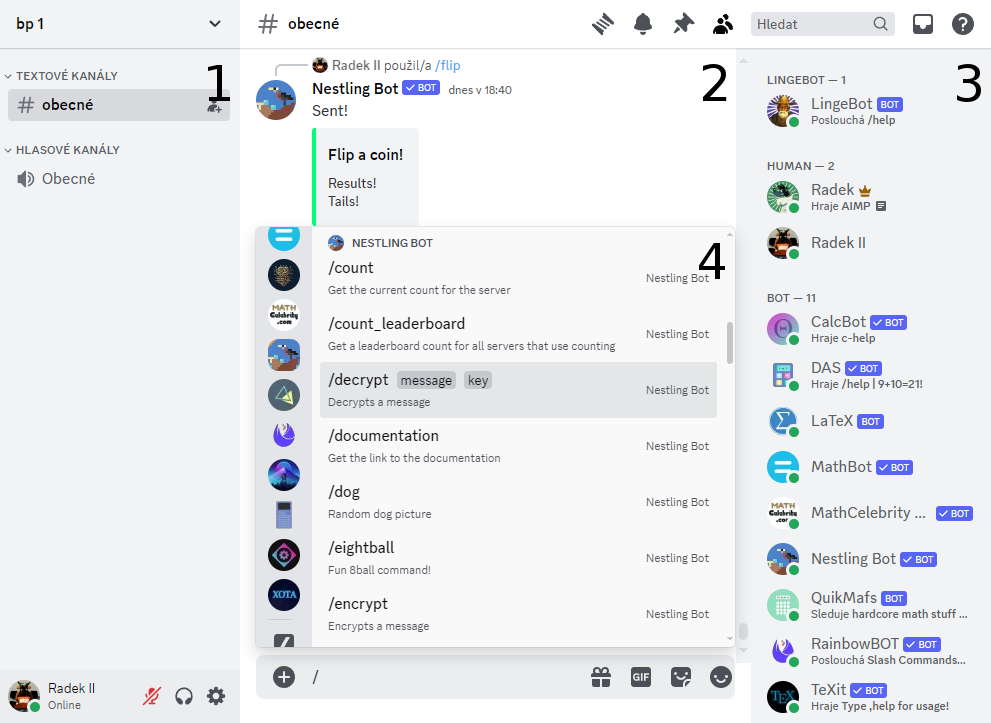
\includegraphics[width=\textwidth]{img/DiscordBotCommands}
		\caption{Discord: Uživatelské rozhraní a použití bota}
	\end{figure}
	
	Boti tedy operují především na serverech, kam jsou pozváni pomocí svého speciálního odkazu (\textit{bot invite link}), lze je ale používat i v přímých zprávách. Bot se sice tváří jako uživatel, do přátel ho ale přidat nelze a pro zahájení přímé konverzace je nutné s ním nejdříve mít nějaký společný server. Bota nelze přidat do soukromé skupiny. 
	
	Discord boti nabízející nástroje pro usnadnění moderace zejména na velkých serverech patří mezi ty nejpoužívanější. Obvykle mají svou stránku s administrací, kde si lze např. zobrazit statistiky serveru, nastavit automatické přivítání a přiřazení rolí novým členům, vyhození za spam apod. Oblíbenou kategorií byli také hudební boti, kteří v hlasové komunikaci pouštěli vybrané skladby. Jejich popularita klesla roku 2021, kdy Google zakázal provoz botů přehrávajících hudbu z webu YouTube. Další častá kategorie botů jsou hry a zábava. Jedná se buď o boty poskytující jednoduché hry v prostředí textového chatu, nebo propojující nějakou existující videohru s Discordem.
	
	\section{Slack}
	
	Z populárních platforem se Discordu vzhledově i funkčně nejvíce podobá program Slack. Ten byl spuštěn již v roce 2013 a od té doby si vybudoval reputaci jako standard pro komunikaci v technologických společnostech. \cite{lit_Discord}
	
	Slack se prezentuje jako software usnadňující interní komunikaci v nějaké organizaci a dal by se nazvat jako \quotedblbase Discord pro firmy\textquotedblleft\,. Namísto serverů jsou zde tzv. workspaces. Workspace má své členy a textové kanály, ve kterých lze zahájit i hlasová komunikace. Členové jednoho workspace si mezi sebou mohou posílat přímé zprávy a pomocí funkce \textit{Slack Connect} je možné komunikovat i s lidmi z jiného workspace. Na rozdíl od Discordu, kde jsou přímé zprávy kompletně oddělené od ekosystému serverů, se zde všechny prováděné akce dějí uvnitř nějakého workspace.
	
	Stejně jako Discord lze Slack používat na webu, desktopu a mobilních zařízeních. Licence je také proprietární. K dispozici je několik verzí měsíčního předplatného a verze zdarma je značně omezena. V bezplatné verzi nelze např. zobrazit zprávy starší než 90 dnů a provozovat hlasovou komunikaci ve více než dvou lidech. Omezené je i použití tzv. aplikací.
	
	Zdejší aplikace (\textit{Apps}) se podobají zkoumaným botům a jejich výběr odpovídá cílové skupině Slacku. Zaměřují se především na zvýšení produktivity, teambuilding, nebo integraci již existující služby třetí strany do prostředí Slacku. Stejně jako uživatelé mohou Slack aplikace spravovat konverzace a odesílat do nich textové zprávy. Ovládání aplikací probíhá buď pomocí příkazů začínajících lomítkem, nebo má každá aplikace svou domovskou stránku a může také generovat vyskakovací okna. Aplikací odeslané zprávy, její domovská stránka a vyskakovací okna mohou obsahovat širokou škálu interaktivních prvků (tlačítko, zaškrtávací pole, výběr data a času apod.).
	
	\begin{figure}[ht]
		\centering
		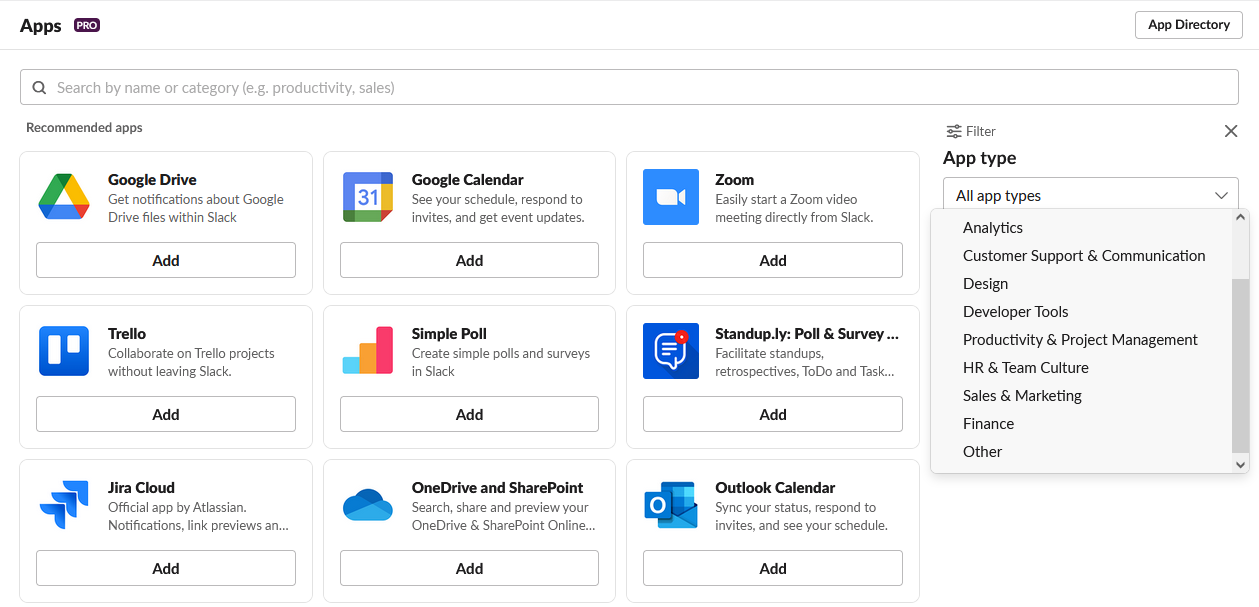
\includegraphics[width=\textwidth]{img/SlackApps}
		\caption{Doporučené Slack aplikace}
	\end{figure}
	
	Zorientovat se v procesu tvorby Slack aplikací nemusí být jednoduché. Tyto aplikace se totiž dělí na klasické (\textit{classic}) a nové (zvané \textit{modern} nebo \textit{next-generation}, představené v roce 2021), jejichž API se liší. Ani slovo bot není ve Slack ekosystému jednoznačné. U klasických aplikací se jedná o jejich speciální typ, se kterým je komunikace vedena běžnou řečí namísto příkazů nebo UI (chatbot). Tento bot je označen jako \textit{legacy} a v budoucnu pravděpodobně nebude podporován. U nového typu aplikací se z pohledu uživatele slovo bot nikde nevyskytuje (maximálně v názvu nějaké aplikace), z dokumentace je ale zjevné, že se (stejně jako u Discordu) jedná o speciálního uživatele ovládaného danou aplikací, tato informace však není nikde explicitně zmíněna. Při práci s dokumentací nebo neoficiálními návody je tedy nutné dávat pozor na to, s jakou technologií daný manuál pracuje, protože může dojít ke snadné záměně výše zmíněných pojmů.
	
	Klasické Slack aplikace lze vyvíjet v řadě komunitních knihoven a musí být hostovány na vlastním serveru. \textit{Next-generation apps} pak mají připravené oficiální \mbox{TypeScript} SDK a o hosting se stará přímo Slack, pro jejich vývoj a následné nasazení je ale nutné mít placenou verzi Slacku.
	
	\section{Guilded a Revolt}
	
	Guilded a Revolt jsou platformy, které jsou přímo inspirované Discordem a podobnost mezi nimi je nepřehlédnutelná. Ekosystém uživatelů, přímých zpráv, serverů a botů je u těchto tří platforem takřka identický. Guilded ani Revolt nemají ekvivalent k podpůrným příkazům. Boti tedy musí kontrolovat obsah každé odeslané zprávy na serveru, jestli neobsahuje nějaký z jejich příkazů. Každý bot má obvykle svůj prefix (např. vykřičník) a problém nastává, když má více botů stejný prefix a příkaz se stejným názvem (např. po napsání \quotedblbase!help\textquotedblleft\ do chatu zobrazí svou nápovědu všichni takoví boti)\footnote{Tímto způsobem se před představením podpůrných příkazů ovládali i boti na Discordu. Problém stejných příkazů se řešil buď víceznakovými prefixy (menší šance na kolizi), nebo nastavitelným prefixem (to vyžaduje nějaké úložiště uchovávající dvojice id serveru a prefix). Tento starý typ příkazů lze stále používat např. pro příkazy, které chce vývojář skrýt před běžnými uživateli (tyto příkazy se neobjeví v našeptávači).}. Obě platformy mají oproti Discordu znatelně menší uživatelskou základnu a počet jejich veřejných botů se pohybuje v řádu desítek.
	
	Guilded (2017) lze považovat za konkurenci Discordu, která se zaměřuje na jeho původní účel. Tím je komunikace pro hráče videoher. Guilded přidává funkcionalitu pro pořádání pravidelných událostí a speciální funkce po propojení účtu s vybranými herními tituly. Licence je proprietární a program je zdarma. Administrátoři ale mohou na svém serveru zapnout dobrovolné měsíční předplatné, ze kterého je část odváděna Guilded. Pro tvorbu botů lze využít komunitních knihoven. \cite{web_guilded}
	
	Revolt (2021) je Discord alternativa s otevřeným zdrojovým kódem. Oproti konkurenci nemá Revolt žádné speciální funkce, díky tomu je ale méně komplikovaný. Kromě řady komunitních knihoven pro tvorbu botů je k dispozici i oficiální revolt.js. Tato knihovna byla vytvořena tak, aby do ní šel snadno migrovat bot napsaný pomocí knihovny discord.js.
	
	\section{Další platformy}
	
	Tato sekce obsahuje\dots
	
	Matrix je otevřený protokol pro šifrovanou komunikaci po síti.
	
	% [Základní popis/Historie, (FEATURES)], [kompatibilita, pricing, licence], [BOTI]
	% Teams
	% flock
	% rocket.chat
	% FB Messenger
	
	\chapter{Matematika na platformě Discord}	
		
	\chapter{Tvorba Discord bota}
	
	\section{Prostředky pro tvorbu}
	
	\section{Návrh}
	
	\section{Implementace}
	
	\section{Zhodnocení}
	
	\chapter{Závěr}
	
	Závěr.
	
	% Zdroje
	\chapter*{Seznam použité literatury}
	\addcontentsline{toc}{chapter}{Seznam použité literatury}
	\printbibliography[heading=none]
	
\end{document}